\documentclass[]{article}
\usepackage{lmodern}
\usepackage{amssymb,amsmath}
\usepackage{ifxetex,ifluatex}
\usepackage{fixltx2e} % provides \textsubscript
\ifnum 0\ifxetex 1\fi\ifluatex 1\fi=0 % if pdftex
  \usepackage[T1]{fontenc}
  \usepackage[utf8]{inputenc}
\else % if luatex or xelatex
  \ifxetex
    \usepackage{mathspec}
  \else
    \usepackage{fontspec}
  \fi
  \defaultfontfeatures{Ligatures=TeX,Scale=MatchLowercase}
\fi
% use upquote if available, for straight quotes in verbatim environments
\IfFileExists{upquote.sty}{\usepackage{upquote}}{}
% use microtype if available
\IfFileExists{microtype.sty}{%
\usepackage[]{microtype}
\UseMicrotypeSet[protrusion]{basicmath} % disable protrusion for tt fonts
}{}
\PassOptionsToPackage{hyphens}{url} % url is loaded by hyperref
\usepackage[unicode=true]{hyperref}
\hypersetup{
            pdfborder={0 0 0},
            breaklinks=true}
\urlstyle{same}  % don't use monospace font for urls
\usepackage[margin=1in]{geometry}
\usepackage{graphicx,grffile}
\makeatletter
\def\maxwidth{\ifdim\Gin@nat@width>\linewidth\linewidth\else\Gin@nat@width\fi}
\def\maxheight{\ifdim\Gin@nat@height>\textheight\textheight\else\Gin@nat@height\fi}
\makeatother
% Scale images if necessary, so that they will not overflow the page
% margins by default, and it is still possible to overwrite the defaults
% using explicit options in \includegraphics[width, height, ...]{}
\setkeys{Gin}{width=\maxwidth,height=\maxheight,keepaspectratio}
\IfFileExists{parskip.sty}{%
\usepackage{parskip}
}{% else
\setlength{\parindent}{0pt}
\setlength{\parskip}{6pt plus 2pt minus 1pt}
}
\setlength{\emergencystretch}{3em}  % prevent overfull lines
\providecommand{\tightlist}{%
  \setlength{\itemsep}{0pt}\setlength{\parskip}{0pt}}
\setcounter{secnumdepth}{0}
% Redefines (sub)paragraphs to behave more like sections
\ifx\paragraph\undefined\else
\let\oldparagraph\paragraph
\renewcommand{\paragraph}[1]{\oldparagraph{#1}\mbox{}}
\fi
\ifx\subparagraph\undefined\else
\let\oldsubparagraph\subparagraph
\renewcommand{\subparagraph}[1]{\oldsubparagraph{#1}\mbox{}}
\fi

% set default figure placement to htbp
\makeatletter
\def\fps@figure{htbp}
\makeatother


\author{}
\date{\vspace{-2.5em}}

\begin{document}

{
\setcounter{tocdepth}{2}
\tableofcontents
}
Preliminary impressions about the relationship between the level of
public debt and the countries ability to attract new foreign credits

Insper Data

Augusto Netto Gabriella Garcia Maria Clara Drzeviechi

\section{Introduction and Motivation}\label{introduction-and-motivation}

This study aims to investigate how a country's level of public debt can
be an obstacle to attract new foreign credits. If the country incurs a
lot of debt, it is more likely that it will not be able to repay its
creditor. Thus, in situations that a country's level of public debt is
too big, the creditors may choose to stop financing the country
(Krugman, 1988), because of the fear of being defaulted.

In the past 50 years, emerging and developing economies experienced four
big indebtedness waves, three of which ended up in financial crises. In
the 1980s, the association of low real interest rates and growing debt
market led certain economies to raise considerably its levels of
indebtedness; the result was the well-known Latin America debt crisis. A
decade later, the world would watch the Asian financial crisis, due to
the liberalization of financial markets and capital flows, allowing
these countries to acquire loans in foreign currencies. Finally, in
2007-09, both emerging and advanced economies faced major recessions as
a result of the Global Financial Crisis.

It is important to notice that although happening in different decades
and locations, these three episodes share a common denominator: they all
started in periods with low real interest rates and an escalating
indebtedness. This scenario made the risk premium rise and subsequently
there was a sudden stop of capital flows.

In 2010, the fourth global wave of debt started, it is worth pointing
out that it was the largest and fastest one. In accordance with the
aforementioned ones, interest rates were low since the Global Financial
Crisis and investors were seeking assets with greater profitability. It
is also reasonable to consider that this wave has not yet met its end.
By 2018, according to the IMF, global debt has reached 226\% of GDP,
representing an amount of 188 trillions of dollars. Emerging and
developing economies saw indebtedness grow 54 p.p.~in 8 years, reaching
170\% of GDP. Low income countries reached 67\% of GDP in 2018, that
figure was 48\% in 2010. A different situation is seen on advanced
economies, once they have maintained the 265\% ratio of debt to GDP on
the same level since 2010.

Considering budget deficits, corporate foreign debt and current account
deficits, one will probably say that the situation in which emerging and
developing countries are now is far worse than that in which they were
in 2010. In addition, part of these economies have since then faced long
periods of low growth and find now a weaker global economy, which puts
them in a more vulnerable situation to external shocks.

Despite low real interest rates, the constant rise in indebtedness can
lead to a sudden rise in risk premia and consequently in interest rates,
aggravating the perspectives of those countries. Something like that has
already been experienced by Argentina and Turkey; both saw a rise in the
cost of servicing the debt.

There is a problem when investors begin to demand a higher premium due
to those higher risks: it can possibly end up in a debt crisis once they
consider a certain Debt/GDP level to be unsustainable (Blanchard 2019;
Henderson 2019; Rogoff 2019a,b). When such a thing happens, it is
expected a flight-to-safety, and weaker and highly indebted economies
see huge capital outflows and a depreciation on the exchange rate.

In this context, this study intends to analyse the impact of the
variable debt-to-GDP ratio on the participation of foreign creditors in
government bonds. Therefore, a worldwide analysis will be conducted
using the database provided by Arslanalp and Takahiro Tsuda, previously
affiliated with the Monetary and Capital Markets Department of the
International Monetary Fund.

\section{Literature Review}\label{literature-review}

Discussions on how indebtedness can affect the macroeconomic variables
of a country are widely addressed in the literature. This review will
focus on three topics: debt and growth; debt overhang and debt
tolerance.

The relationship between debt and growth was first found to be
non-linear by Reinhart, Rogoff, and Savastano (2003). Later, Reinhart
and Rogoff (2010) analyze countries distinguishing developed and
emerging markets and they found out that, for both groups, a 90\% debt
to GDP ratio can be detrimental for growth. On the other hand, Kumar and
Woo (2010) produced evidence that the negative impact of debt on growth
is higher for developing countries when compared with developed
countries.

Thinking about debt tolerance, Reinhart, Rogoff and Savastano (2003)
introduce the concept of debt intolerance and analyze how emerging
markets find it difficult to face high levels of debt, while advanced
countries face this issue more easily. Later, Catão and Kapur (2006)
discussed the macroeconomic determinants of a country's volatility and
how it impacts the spread rate it has to pay.

The concept of debt overhang refers to a debt burden so large that the
country can not take any additional debt to finance itself. Krugman
(1988) discussed the tradeoff for creditors when facing a debt overhang:
financing or forgiving. Deshpande (1995) discusses how a situation of
debt overhang can discourage investment. Reinhart, Reinhart, and Rogoff
(2012) punctuated the main episodes in history about debt overhang.

\section{Dataset Description}\label{dataset-description}

Initially, the dataset used in this study is composed by the database
provided by Arslanalp and Takahiro Tsuda and the World Economic Outlook
from IMF. The dataset is composed of 45 countries sixteen years.

\begin{verbatim}
##     country  yearQ year quarter total_debt_ debt_to_GDP_       fx_
## 1 Argentina 2004Q4 2004       4    436.7520     94.48977 0.3420390
## 2 Argentina 2005Q4 2005       4    371.5375     68.84866 0.3430018
## 3 Argentina 2006Q4 2006       4    463.2258     69.82613 0.3264318
## 4 Argentina 2007Q4 2007       4    496.1755     60.72736 0.3222925
## 5 Argentina 2008Q4 2008       4    527.6820     49.75965 0.3156896
##   nonbank_domestic_debt_ bank_domestic_debt_ official_domestic_debt_
## 1               88.30325            97.28225                248.1838
## 2               67.04950           101.18550                225.0013
## 3              157.65575            91.15900                302.0340
## 4              165.31975            90.76500                312.1260
## 5              188.12300            92.74625                344.1098
##   domestic_debt_ nonbank_foreign_debt_ bank_foreign_debt_
## 1       248.1838             128.08725            1.04150
## 2       225.0013              91.30875            0.74575
## 3       302.0340             107.93475            0.86425
## 4       312.1260             136.42225            1.12525
## 5       344.1098             131.57650            0.81425
##   official_foreign_debt_ foreign_debt_ woe_country_code GDP_cte GDP_cur
## 1               59.43975      188.5680              213    8911  482220
## 2               54.48125      146.5362              213    8852  541253
## 3               52.39350      161.1925              213    8047  602507
## 4               46.50200      184.0493              213    9008  674423
## 5               51.18125      183.5720              213    4057  715435
##   GDP_per_cap_cte inflation_mean inflation_end unemployment
## 1            7896           4416          6101        13625
## 2            7819           9642         12327        11575
## 3            6998          10898          9841        10175
## 4            7939           8830          8468         8475
## 5            3038           8585          7238         7875
##   lending_borroeing_rate account_balance develop    taxes  vix_EUA  vix_EUR
## 1               3967.000            1798      EM 18.88978 15.45679 18.88630
## 2               3341.000            2473      EM 19.82989 12.77985 14.03113
## 3               1650.000            2791      EM 18.66199 12.78038 16.52675
## 4                  0.757            2100      EM 14.23548 17.45257 19.61443
## 5                  0.352            1492      EM 13.08275 32.58267 33.70876
##   Scale nominal_rate     continent GDP_per_cap_cur_USD
## 1 Units         2.50 South America            4277.721
## 2 Units         5.00 South America            5109.851
## 3 Units         6.25 South America            5919.012
## 4 Units        10.75 South America            7245.448
## 5 Units        12.05 South America            9020.873
\end{verbatim}

\section{Stylized Facts}\label{stylized-facts}

Firstly, some stylized facts will be explained in relation to our
dataset.

\subsection{The level of indebtedness in the world has varied
considerably in recent
years}\label{the-level-of-indebtedness-in-the-world-has-varied-considerably-in-recent-years}

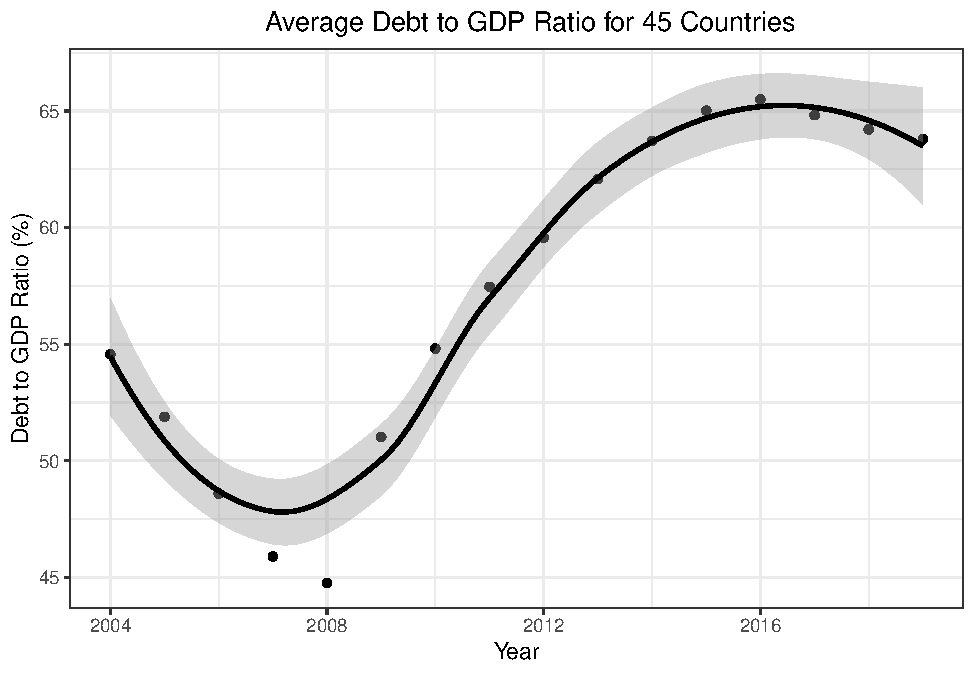
\includegraphics{Insper_Data_Macro_Project_Sep_files/figure-latex/unnamed-chunk-2-1.pdf}

It is possible to observe that the average indebtedness in the countries
fell a lot in 2008, rise until 2018 and has been showing a slight drop.

\subsection{Advanced markets are more indebted than emerging
markets}\label{advanced-markets-are-more-indebted-than-emerging-markets}

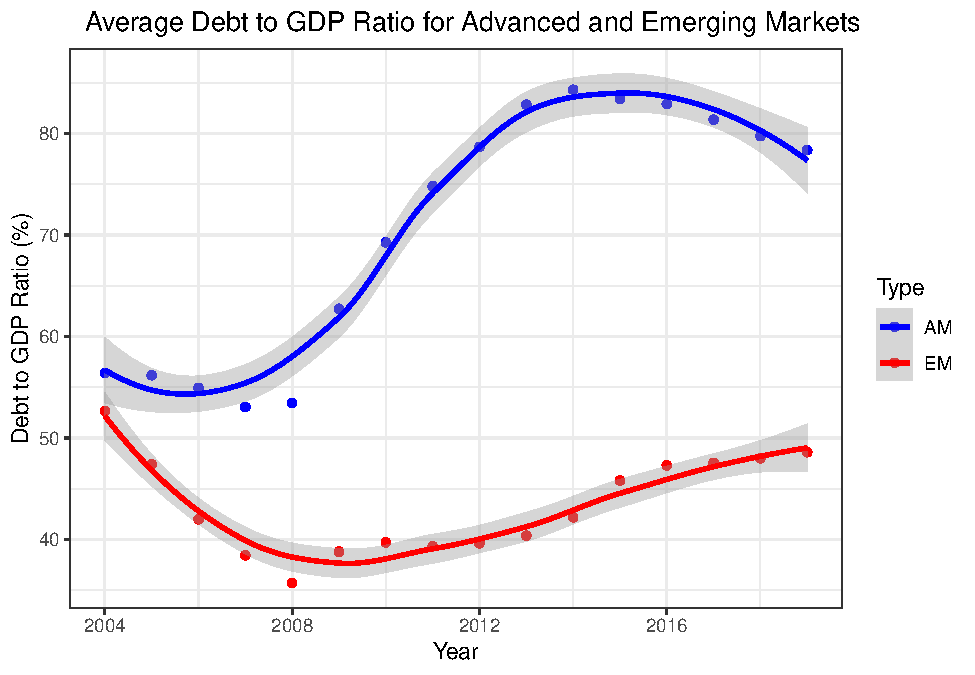
\includegraphics{Insper_Data_Macro_Project_Sep_files/figure-latex/unnamed-chunk-3-1.pdf}

\subsection{The relationship between debt and GDP is not
clear}\label{the-relationship-between-debt-and-gdp-is-not-clear}

\end{document}
